\documentclass[a4paper, fontsize=14pt]{scrartcl}
\usepackage{cmap} % сразу после \documentclass
\usepackage[left=3cm,right=1.5cm,top=2cm,bottom=2cm]{geometry}
\usepackage{indentfirst}
\setlength{\parindent}{1.25cm} % для шрифта 14pt
\setcounter{page}{2} % нумерация страниц начнётся с 2
\usepackage{setspace}
\onehalfspacing
\textheight=24cm % высота текста

\usepackage[]{cite}
\usepackage[T2A]{fontenc}
\usepackage[utf8]{inputenc}
\usepackage[english, russian]{babel}
\usepackage{amsmath, amsfonts, amssymb, amsthm}
\usepackage{graphicx, epsfig}
\graphicspath{{pictures/}}
\DeclareGraphicsExtensions{.pdf,.png,.jpg}
\usepackage{subfig}
\usepackage{color}
\usepackage{gensymb}
 
\usepackage{enumitem}	
\setlist{nolistsep} 


\usepackage{algorithm}
\usepackage{algpseudocode}
\floatname{algorithm}{Алгоритм}
\algnewcommand{\IIf}[1]{\State\algorithmicif\ #1\ \algorithmicthen}
\algnewcommand{\EndIIf}{\unskip\ \algorithmicend\ \algorithmicif}
\renewcommand{\algorithmicend}{\textbf{завершим}}
\renewcommand{\algorithmicif}{\textbf{если}}
\renewcommand{\algorithmicelse}{\textbf{иначе}}
\renewcommand{\algorithmicthen}{\textbf{то}}
\renewcommand{\algorithmicdo}{\textbf{выполним}}
\renewcommand{\algorithmicfor}{\textbf{цикл для}}
\renewcommand{\algorithmicforall}{\textbf{цикл для всех}}
\renewcommand{\algorithmicwhile}{\textbf{цикл пока}}




\usepackage{hyperref}
\usepackage [section] {placeins}


\begin{document}
\author{Черненков Алексей Юрьевич}

\addcontentsline{toc}{section}{\protect\numberline{}Аннотация}
\section*{Аннотация}
\begin{abstract}

Получена модель для расчета альбедо снега, учитывающая изменения основных его параметров. Определены основные факторы, влияющие на величину альбедо заснеженной поверхности, получены зависимости, описывающие их изменения. Модифицирован почвенно-снежный блок глобальной климатической модели ИВМ РАН, в результате чего улучшено описание площади, покрытой снегом. Полученные результаты можно использовать для внедрения блока расчета альбедо снега в модель климата. Другим приложением полученной модели является задача оценки радиационного форсинга от загрязнения снега атмосферными аэрозолями. 
  
  \bigskip
  \textbf{Ключевые слова}: \emph{климат, климатическая модель, альбедо снега, метаморфизм снега, черный углерод, радиационная модель, радиационный форсинг}
\end{abstract}


\newpage
\phantomsection
\addcontentsline{toc}{section}{\protect\numberline{}Содержание}
\tableofcontents


\newpage
\section*{Введение}
\addcontentsline{toc}{section}{\protect\numberline{}Введение}

В течении последних десятилетий набирают актуальность вопросы, связанные с изменениями климата. Для предсказания будущих изменений активно используются климатические модели. Большинство из них представляют собой совместно работающие модели общей циркуляции атмосферы и океана, дополненные другими блоками, описывающими отдельные процессы, протекающие внутри климатической системы, например, углеродный цикл. Работа таких моделей требует значительных вычислительных ресурсов. Рост доступных вычислительных мощностей позволяет более подробно описывать процессы на Земле, повышая общую точность модели. 

Одной из важнейших переменных в моделях климата является альбедо. Данная величина характеризует отражающие свойства поверхности по отношению к солнечной радиации. Альбедо участвует в описании радиационного баланса Земли, его уменьшение приводит к дополнительному нагреву поверхности. В случае снега падение данной величины может быть вызвано, например, загрязнением различными примесями.

Целью данной работы было получение модели альбедо заснеженной поверхности, которую можно было бы как использовать для отдельных локальных расчетов, так и внедрить в глобальную климатическую модель, например, INMCM5 \cite{Volodin2017}.  

В текущей версии климатической модели ИВМ РАН реализована простая параметризация заснеженной поверхности на суше, зависящая только от температуры поверхности $T$ \cite{sysAlbOld}. 
\begin{equation}
    \alpha_{sn} = \begin{cases}
                        0.8,~ T \leq -1 ~\degree \mathrm{C}; \\
                        0.8 - 0.1(T + 1), ~T > -1 ~\degree \mathrm{C};
                  \end{cases} \label{sysAlbOld}
\end{equation}
В сравнении с другими моделями альбедо из модели INMCM5 несколько занижено, например, \cite{Flanner2007, Gueymard2019}, поэтому использование более подробного описания данной величины потенциально может уточнить модель.

\newpage
\begin{figure}[h]
    \center{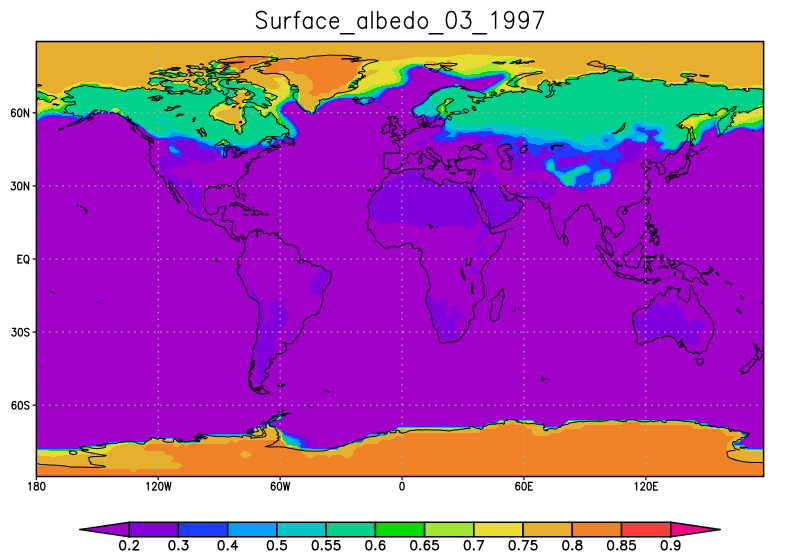
\includegraphics[scale=0.5]{Surface_albedo_03_1997.png}}
    \caption{Среднемесячное альбедо по данным модели INMCM5 (март 1997 г.)}
    \label{fig:imageAlbOld}
\end{figure}


Другим актуальным приложением модели альбедо является задача расчета радиационного форсинга от загрязнения заснеженной поверхности примесями. Выпадая на снег, они изменяют его оптические свойства, что приводит к дополнительному нагреву планеты. Оценку этого нагрева можно получить, рассматривая изменение альбедо. 

Побочным результатом данной работы стала модернизация почвенно-снежного блока климатической модели ИВМ РАН. Была уточнена реализация процесса таяния снега, а также реализованы процесс перезамерзания талой воды и описание эволюции плотности снежного слоя. Данные изменения способствуют более точному описанию снежного покрова в переходные сезоны, а также позволили уточнить описание площади, покрытой снегом.

Отдельные результаты магистерской диссертации изложены в статье \cite{Chernenkov2021rus} и сборниках докладов \cite{MSARD2019, mipt2019, EGU2020poster, EGU2020, mipt2020, Arctic2020}, а также докладывались и обсуждались на следующих научных конференциях, в том числе с международным участием:
\begin{itemize}
    \item Международный симпозиум «Атмосферная радиация и динамика» (МСАРД–2019), 25 – 27 июня 2019, Санкт-Петербург \cite{MSARD2019}
    \item 62-я Всероссийская научная конференция МФТИ, секция ФПМИ – Вычислительные технологии и моделирование, Москва, 2019 \cite{mipt2019}
    \item EGU2020: Sharing Geoscience Online, ITS2.15/BG2.25 Pan-Eurasian Experiment (PEEX) – Observation, Modelling and Assessment in the Arctic-Boreal Domain, May, 2020 \cite{EGU2020poster, EGU2020} \sloppy 
    \item 63-я Всероссийская научная конференция МФТИ, Секция ФПМИ – Вычислительные технологии и моделирование, Москва, 2020 \cite{mipt2020}
    \item Вторая Всероссийская научная конференция «Мониторинг состояния и загрязнения окружающей среды. Экосистемы и климат Арктической зоны». Москва, 25-27 ноября 2020 \cite{Arctic2020}
\end{itemize} 



\newpage
\section{Постановка задачи}

Главной задачей данной работы было построение модели альбедо заснеженной поверхности, которая учитывала бы его зависимости от основных параметров, а также была бы пригодна для внедрения в глобальную климатическую модель, например, INMCM5 \cite{Volodin2017}. Стоит отметить, что модель альбедо строилась для случая достаточно толстого слоя снега (не менее 10 см). Данное предположение обусловленно тем, что в случае более тонкого слоя значительную роль начинает играть альбедо подстилающей поверхности, что сильно усложняет задачу. 

На первом этапе было необходимо определить основные факторы, от которых зависит снежное альбедо. Таковыми оказались: солнечное склонение, наличие в слое снега примесей, а также его структура: форма и размеры снежных кристаллов.

Следующим шагом было получение зависимостей, описывающих основные характеристики альбедо. Для этого было необходимо построить:
\begin{itemize}
    \item зависимость, описывающую изменение солнечного зенитного угла в течении астрономического года,
        \item технологию расчета концентраций примесей, содержащихся в слое снега,
        \item модель, описывающую снежный метаморфизм.
\end{itemize} 

В ходе изучения метаморфизма снега выяснилось, что в климатической модели ИВМ РАН отсутствуют несколько переменных, необходимых для его описания. Так как модель альбедо строилась с учетом совместного использования с данной глобальной моделью, то возникла задача модификации почвенно-снежного блока модели ИВМ. Было необходимо ввести новые прогностические переменные, описывающие жидкую воду в слое снега, а также лед, образовавшийся в результате перезамерзания талой воды. Также требовалось реализовать расчет плотности слоя снега с учетом данных параметров.

В целом, результатов, полученных на предыдущих этапах, достаточно для проведения расчетов альбедо по данным климатической модели ИВМ РАН, например, с помощью радиационной модели SNICAR \cite{Flanner2007}. Однако, в таком случае расчеты возможны только на этапе обработки данных, а хотелось бы иметь возможность проводить их на каждом шаге по времени внутри модели. Внедрение модели SNICAR в климатическую модель ИВМ сопряжено со сложностями различного характера, поэтому следующим этапом стало построение параметризации альбедо на основании модели SNICAR. 

Заключительным шагом было применение построенной модели альбедо для оценки радиационного форсинга от загрязнения снега черным углеродом. Таким образом, данная модель тестировалась на реальной задаче. 


\newpage
\section{Факторы, влияющие на альбедо снега}
Альбедо -- это физическая величина, равная отношению отраженной от поверхности радиации к падающей. Например, для свежевыпавшего сухого снега альбедо составляет $0.85-0.95$, для лежалого загрязненного снега уже $0.40-0.50$, для морского льда $0.30-0.40$, а для древесного угля примерно $0.04$. Данная величина играет важную роль в радиационном балансе. Ее уменьшение приводит к увеличению поглощения поверхностью приходящей радиации, что влечет за собой дополнительный нагрев планеты. 

Основными факторами, влияющими на отражающую способность снега являются форма и размеры снежных кристаллов, наличие различных примесей в снегу, в частности, черного углерода \cite{Bak2019}. Также важно отметить, что альбедо зависит от угла, под которым на поверхность Земли приходит солнечная радиация. Далее опишем каждый из этих факторов.


\subsection{Солнечный зенитный угол}

Значение солнечного склонения меняется в течении года из-за движения Земли по эллиптической орбите вокруг Солнца и наклона ее собственной оси вращения. Так, он равен нулю два раза в год: в дни весеннего и осеннего равноденствия. В результате из-за этого меняется солнечный зенитный угол, под которым на поверхность Земли приходит излучение, что непосредственно влияет на величину альбедо. Особенно сильное влияние данное явление оказывает в случае верхних широт. 

Косинус зенитного угла для северного полушария выражается через угол склонения Солнца и широту местности следующим образом: пусть $\delta$ –- угол склонения Солнца, $\phi$ –- широта, $\theta$ –- солнечный зенитный угол, тогда:
\begin{equation}
    \cos \theta = \cos ( \phi - \delta ) \label{sys}
\end{equation}
при этом:
\begin{equation}
    \sin \delta = \sin \varepsilon \sin \left(\dfrac{2 \pi (d - d_e)}{365} \right) ,  \label{sys}
\end{equation}
где $\varepsilon$ = 23.45$\degree$  – наклон Земли к плоскости эклиптики, $d$ – время (в сутках с начала года), $d_e$ = 80.5.


\begin{figure}[h]
    \begin{minipage}[h]{0.49\linewidth}
        \center{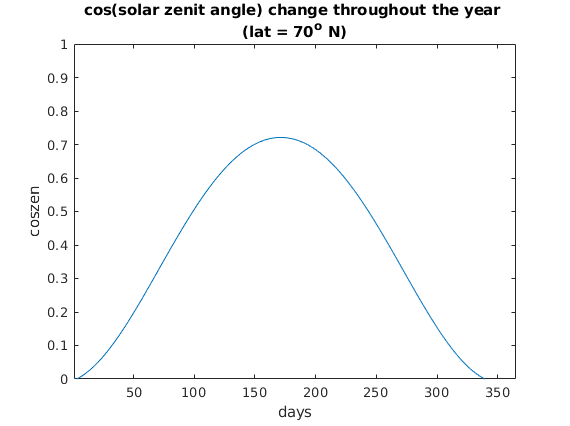
\includegraphics[width=1.1\linewidth]{coszen2.png} \\ (а)}
    \end{minipage}
    \hfill
    \begin{minipage}[h]{0.49\linewidth}
        \center{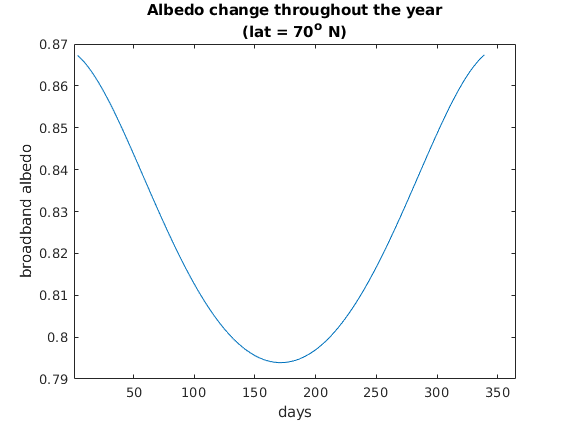
\includegraphics[width=1.1\linewidth]{coszen3.png} \\ (б)}
    \end{minipage}
    \caption{Изменения (а) косинуса солнечного зенитного угла и (б) альбедо в течении года (при остальных фиксированных условиях), вызванные вращением Земли вокруг Солнца (на примере точки, находящейся на $70\degree$ С.Ш.)}
    \label{fig:image}
\end{figure}


\subsection{Метаморфизм снега}

С течением времени после снегопада из-за изменений температуры, а также под действием давления снежные кристаллы изменяют свою форму от изначально очень сложных (например, фрактальная "Снежинка Коха") до близкой к сферической, а также увеличиваются в размерах, слипаясь \cite{Grenfell1999, Grenfell2005, He2018}. Это приводит к уменьшению отражающей способности заснеженной поверхности, что особенно заметно в случае длин волн, относящихся к ближнему ИК-диапазону ($0.7-5.0$ мкм). Другим важным фактором для описания метаморфизма является наличие в слое снега жидкой воды и перезамерзших кристаллов. Наличие таких фракций в слое снега также приводит к уменьшению альбедо. Это наиболее явно проявляется в переходные сезоны, когда происходит активное таяние или, наоборот, формирование снежного покрова.

\begin{figure}[h]
    \begin{minipage}[h]{0.5\linewidth}
        \center{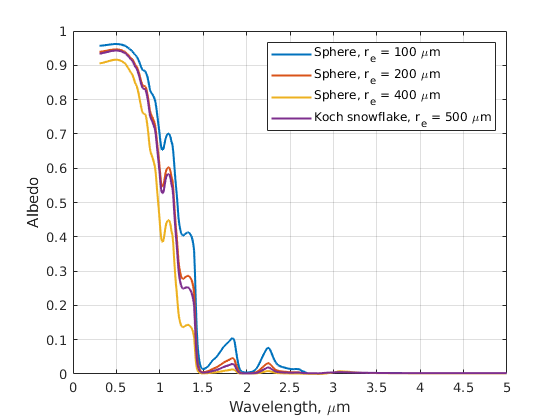
\includegraphics[width=1\linewidth]{rds3.png} \\ (а)}
    \end{minipage}
    \hfill
    \begin{minipage}[h]{0.5\linewidth}
        \center{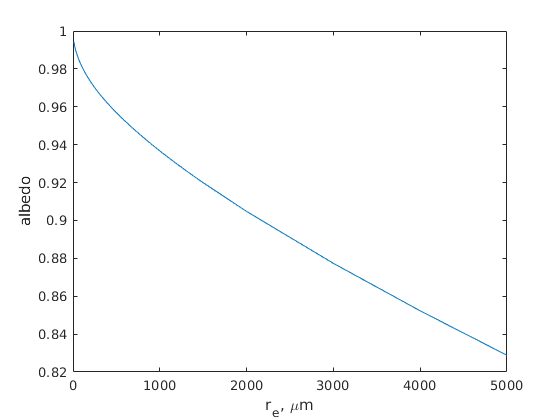
\includegraphics[width=1\linewidth]{rds2.png} \\ (б)}
    \end{minipage}
    \caption{(а) Спектральное альбедо, соответствующее различным формам и размерам снежного кристалла, и (б) зависимость альбедо от эффективного радиуса снежного кристалла}
    \label{fig:image}
\end{figure}

\newpage
Для описания снежных кристаллов с достаточно хорошей точностью можно применять приближение, использующее ледяные шарообразные частицы, сохраняющие удельную площадь поверхности ($SSA$) (в том числе, в случаях кристаллов сложных форм) \cite{Grenfell1999}. Их основная характеристика -- эффективный радиус ($r_e$). Он определяется как средневзвешенный по площади радиус ансамбля таких частиц и связан с удельной площадью поверхности ($SSA$) и плотностью льда $\rho_{ice}$ следующим образом \cite{Flanner2006}:  
\begin{equation}
    r_e = \dfrac{3} {\rho_{ice} \cdot SSA} \label{sys}
\end{equation}
Таким образом, старение снега можно описывать как эволюцию эффективного радиуса снежного кристалла. Рассмотрим зависимость, использованную в климатической модели CLM4.5 \cite{CLM4.5tech}. Пусть момент времени $t$ соответствует текущему шагу по времени, а $(t - 1)$ -- предыдущему. Тогда старение снега можно описать следующим уравнением:
\begin{equation}
    r_e(t) = [r_e (t - 1) + \delta r_{e , dry} + \delta r_{e , wet} ] \cdot f_{old} + r_{e ,0} \cdot f_{new} + r_{e , rfz} \cdot f_{rfrz}, \label{sysRDS1}
\end{equation}
где $ r_{e ,0} = 54.5 $ мкм и $r_{e , rfz} = 1000 $ мкм -- значения эффективного радиуса, соответствующие свежевыпавшему и перезамерзшему снегу, $\delta r_{e , dry}$ и $\delta r_{e , wet}$ -- вклады от метаморфизма сухого и мокрого снега, $f_{old}$, $f_{new}$ и $f_{rfrz}$ -- доли лежалого, свежевыпавшего и перезамерзшего снега соответственно.  

Эволюция сухого снега описывается следующим уравнением \cite{Flanner2006, Flanner2007, CLM4.5tech}:
\begin{equation}
    \dfrac{d}{dt} \delta r_{e , dry} = {\left( \dfrac{dr_{e , dry}}{dt} \right)}_0 \left(\dfrac{\eta}{\eta + (r_e - r_{e, 0})}\right)^{1 / \kappa}, \label{sys}
\end{equation}
где ${\left( \dfrac{dr_{e , dry}}{dt} \right)}_0$, $\eta$, $\kappa$ -- некоторые табличные параметры, зависящие от температуры снега $T$, температурного градиента $\dfrac{dT}{dz}$ и плотности снега $\rho_{sn}$, причем для каждого значения $SSA$ они различные. Эти данные находятся в открытом доступе (\url{http://snow.engin.umich.edu/snowaging/}). Они охватывают следующие диапазоны параметров: по температуре от $-50$ до $0 ~\degree$C, по плотности от $50$ до $400$ кг$/$м$^3$, по температурному градиенту от $0$ до $300$ К$/$м для следующего набора значений $SSA$: $60$, $80$, $100$ м$^2/$кг. В работах \cite{CLM4.5tech, Flanner2006, Flanner2007} предлагается считать $SSA = 60$ м$^2/$кг.

Эволюция мокрого снега описывается следующим эмпирическим уравнением \cite{CLM4.5tech, Brun1989}:
\begin{equation}
\dfrac{d}{dt} \delta r_{e , wet} = \dfrac{C \cdot f_{liq}^3} {4 \pi r_{e}^2}, \label{sys}
\end{equation}
где $C = 4.22 \cdot 10^{5}$ мкм$^3/$c, $f_{liq}$ -- доля жидкой воды в снегу.

Учитывая, что нас интересует суммарный вклад и от сухого, и от мокрого снега, предыдущие два уравнения можно объединить в одно. Считая начальным значением эффективного радиуса его величину с прошлого шага по времени, получаем следующую задачу Коши для суммарного вклада:
\begin{equation}
    \begin{cases}
        \dfrac{d}{dt} \delta (r_{e , dry} + r_{e , wet}) = {\left( \dfrac{dr_{e , dry}}{dt} \right)}_0 \left(\dfrac{\eta}{\eta + (r_e - r_{e, 0})}\right)^{1 / \kappa} + \dfrac{C \cdot f_{liq}^3} {4 \pi r_{e}^2} ,
        \\
        \delta (r_{e , dry} + r_{e , wet})(t_0) = 0; 
    \end{cases} \label{sysRDS2}
\end{equation}
где $t_0 = t - 1$. 

\newpage
Данное дифференциальное уравнение решалось численно с помощью явного метода Эйлера.

\begin{figure}[h]
    \center{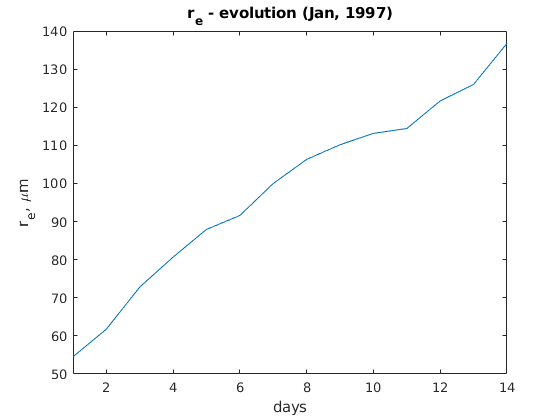
\includegraphics[scale=0.85]{rds1.png}}
    \caption{Эволюция эффективного радиуса снежного кристалла за первые 2 недели января, рассчитанное с использованием описанной выше зависимости}
    \label{fig:image}
\end{figure}
 

\subsection{Загрязнение снега атмосферными аэрозолями}

Выпадение на заснеженную поверхность атмосферных аэрозолей приводит к ее загрязнению и, как следствие, уменьшению ее отражающей способности (до $25 \%$). Наибольшее влияние оказывают такие аэрозоли как минеральная пыль и черный углерод (ЧУ) или сажа. Основными источниками сажевого аэрозоля являются выбросы, возникающие при сжигании различных видов топлива, а также лесные и степные пожары. В качестве меры загрязнения можно рассматривать концентрацию примеси в слое снега. Опишем технологию расчета такой концентрации на примере черного углерода.



\begin{figure}[h]
    \center{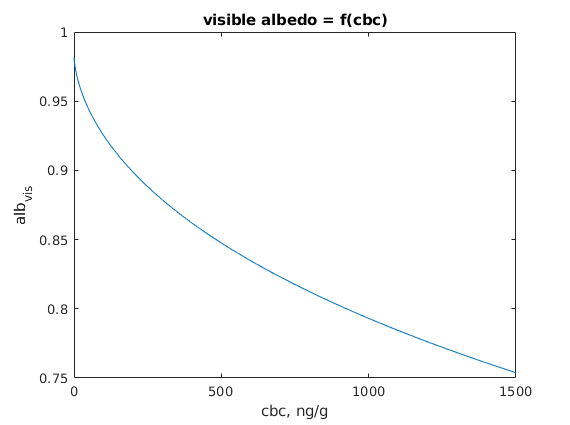
\includegraphics[scale=0.9]{alb_cbc.png}}
    \caption{Зависимость снежного альбедо от концентрации ЧУ в снегу}
    \label{fig:image}
\end{figure}

\newpage
Пусть имеются следующие климатические данные:
\begin{itemize}
    \item $H_{snw}$ -- водно-эквивалентная толщина снега, 
    \item $I_{bc}$ -- поток черного углерода на поверхности снежного слоя, 
    \item $Q_{melt}$ -- поток талой воды на нижней границе снежного слоя,
    \item $\sigma$ -- доля ячейки сетки, покрытая снегом.
\end{itemize}


\\~

Дополнительно предположим, что имеет место равномерное перемешивание частиц атмосферного аэрозоля и снежных гранул. Необходимо также отметить, что в рассматриваемой модели снег предполагается однослойным. Данное замечание важно, так как в реальности основная часть аэрозоля не проникает вглубь снежного покрова, а остается в его верхних слоях.

\newpage
Рассмотрим следующие промежуточные поля за $n$-ый месяц, необходимые для вычисления среднемесячной концентрации ЧУ в снегу: 
\begin{itemize}
    \item приток массы ЧУ в ячейке, покрытой снегом:
    \begin{equation}
        P_{bc}^n = I_{bc}^n \Delta t \sigma^n S   \label{sys}
    \end{equation}
    \item масса снега в ячейке сетки:
    \begin{equation}
        M_{sn}^n = H_{snw}^n \rho_w S   \label{sys}
    \end{equation}
\end{itemize} 
Здесь $\rho_w = 1000$ кг/м$^3$ -- плотность воды, $S$ –- площадь ячейки сетки, $\Delta t = 1$ месяц.
    
Массу ЧУ в заснеженной ячейке сетки $M_{bc}$ можно рассчитать на основе балансового соотношения, предложенного в работе \cite{Flanner2007}:

\begin{equation}
    \dfrac{d M_{bc}}{d t} = - C_{MSE} ~ Q_{melt} ~ \dfrac{M_{bc}}{M_{sn}} ~ S + I_{bc} ~ \sigma S     \label{sysBalanceCount}
\end{equation}
Данная зависимость описывает изменение массы ЧУ в слое снега из-за вымывания его талой водой и притока за счет осаждения на поверхность частиц атмосферного аэрозоля. Соотношение ($\ref{sysBalanceCount}$) можно переписать в дискретном виде следующим образом:

\begin{equation}
   M_{bc}^{n+1} = M_{bc}^n - C_{MSE} ~ Q_{melt}^{n+1} ~ \dfrac{M_{bc}^n}{M_{sn}^n} ~ S \Delta t + P_{bc}^{n+1}     \label{sysBalance}
\end{equation}
Здесь $Q_{melt} = - \dfrac{1}{S} \dfrac{dM_{sn}}{dt} \geq 0$ --  средний по ячейке поток массы растаявшего снега, $C_{MSE}$ -- коэффициент вымывания частиц ЧУ талой водой. Если считать, что поток ЧУ из атмосферы $I_{bc}^{n + 1} = 0$, то из прошлого уравнения следует, что:

\begin{equation}
   C_{MSE} = \dfrac{\Delta M_{bc} / M_{bc}}{\Delta M_{sn} / M_{sn}}     \label{sys}
\end{equation}
Таким образом, с физической точки зрения коэффициент $C_{MSE}$ –- это отношение вымываемой относительной массы ЧУ к относительной
массе талой воды. Для гидрофильного черного углерода $C_{MSE} = 0.2$, для гидрофобного $C_{MSE} = 0.03$ \cite{Flanner2007, Conway1996}. В расчетах с временными масштабами порядка месяца с хорошей точность можно считать весь черный углерод гидрофильным, так как характерное время его перехода в такое состояние из гидрофобного составляет порядка 2 дней.

В качестве начальных данных для дискретного балансового уравнения \eqref{sysBalance} можно использовать следующее выражение:
\begin{equation}
    M_{bc}^0 = P_{bc}^0, \label{sysStart}
\end{equation}
где нулевой индекс означает месяц, когда в данной ячейке сетки появился снежный покров. 

Зная решение задачи \eqref{sysBalance}, \eqref{sysStart}, можно найти среднемесячную концентрацию ЧУ в снегу по следующей формуле:
\begin{equation}
   C_{bc}^n = \dfrac{M_{bc}^n}{M_{sn}^n}  \label{sys}
\end{equation}

\begin{figure}[h]
    \center{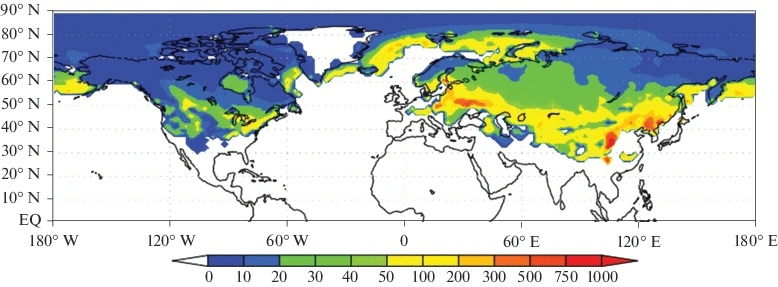
\includegraphics[scale=0.6]{Cbc1.jpg}}
    \caption{Среднемесячная концентрация черного углерода в снегу, рассчитанная по данным климатической модели ИВМ РАН (январь 1998 г.), [нг/г]}
    \label{fig:image}
\end{figure}

Таким образом, получена технология для расчета концентрации примесей в снегу. Причем, ее можно использовать как на этапе обработки климатических данных, так и внутри глобальной модели. Отдельно нужно отметить, что данная модель позволяет проводить расчетов как для снежного покрова на суше, так и для снега на океаническом льду.

Стоит отметить, что результаты расчетов концентрации черного углерода в снегу с использованием описанной технологиии хорошо согласуются с результатами других опубликованных работ, например, \cite{Flanner2007}.

\newpage
\section{Модификация глобальной климатической модели ИВМ РАН}

\subsection{Общие сведения о климатической модели ИВМ РАН}

Рассматривается пятая версия климатической модели ИВМ РАН (INMCM5) \cite{Volodin2017rus}. Она представляет собой модель совместной общей циркуляции атмосферы и океана, дополненную аэрозольным блоком. Данная версия имеет разрешение по долготе--широте $2 \times 1.5\degree$ в атмосфере и $0.5 \times 0.25\degree$ в океане. По высоте в атмосфере она содержит 71 уровень, а океане -- 40 уровней. \sloppy

Атмосферный блок представляет собой численное решение системы уравнений гидротермодинамики в приближении гидростатики. Для решения системы применяется конечно-разностная схема, которая имеет второй порядок по пространству и первый порядок по времени. Основными прогностическими переменными данной модели являются горизонтальные составляющие ветра, температура, удельная влажность и приземное давление. 

Данная версия модели участвует в международном проекте по сравнению климатических моделей CMIP6 (Coupled Models Intercomparison Project). Некоторые результаты по моделированию современного климата с помощью данной модели представлены в работе \cite{Volodin2017rus}.  \sloppy 


\subsection{Описание почвенно-снежного блока модели}

Для совместного использования климатической модели ИВМ РАН и модели, описывающей метаморфизм снега\eqref{sysRDS1, sysRDS2}, и последующего расчета альбедо снега были необходимы изменения в почвенно-снежном блоке модели общей циркуляции атмосферы, поэтому кратко опишем его \cite{Volodin1998, Volodina2000}.   

\newpage
Определим необходимые переменные:
\begin{itemize}
    \item $t$ -- время, 
    \item $z$ -- вертикальная координата (напрвлена вниз), 
    \item $T$ -- температура, 
    \item $W$ -- количество жидкой влаги, 
    \item $V$ -- количество водяного пара, 
    \item $I$ -- количество льда, 
    \item $\lambda_T$ -- коэффициент теплопроводности, 
    \item $\lambda_W$ и $\lambda_V$ -- коэффициенты диффузии воды и водяного пара, 
    \item $\delta$ -- коэффициент термо-влагопроводности, вызванной температурным градиентом, 
    \item $\rho$ и $C$ -- плотность и теплоемкость почвы, 
    \item $\gamma$ -- скорость инфильтрации воды под действием силы тяжести, 
    \item $L_i$ -- удельная теплота плавления льда, 
    \item $L_v$ -- удельная теплота парообразования, 
    \item $F_i$ -- скорость изменения количества жидкой влаги и льда при замерзании / таянии, 
    \item $F_v$ -- скорость изменения содержания водяного пара и воды при испарении, 
    \item $R_f$ -- изменение влагосодержания из-за горизонтального стока воды, 
    \item $R_r$ -- скорость всасывания воды корневой системой растительности.
\end{itemize} 

\\~

В климатической модели ИВМ РАН данный блок представлен одномерной моделью, которая описывает процессы тепло- и влагопереноса в почве и снежном покрове, а также обмен этой системы теплом и влагой с атмосферой. Основой для данной модели является численное решение следующей системы уравнений:

\begin{equation}
    \rho  C \dfrac{\partial T}{\partial t} = \dfrac{\partial }{\partial z} \lambda_T \dfrac{\partial T}{\partial z} + L_i F_i - L_v F_v  \label{sys1}
\end{equation}
\begin{equation}
    \dfrac{\partial W}{\partial t} = \dfrac{\partial }{\partial z} \lambda_W \left( \dfrac{\partial W}{\partial z} + \delta \dfrac{\partial T}{\partial z} \right) + \dfrac{\partial \gamma}{\partial z} - F_i - F_v - R_f - R_r  \label{sys2}
\end{equation}
\begin{equation}
    \dfrac{\partial V}{\partial t} = \dfrac{\partial }{\partial z} \lambda_V \dfrac{\partial V}{\partial z} + F_v  \label{sys3}
\end{equation}
\begin{equation}
    \dfrac{\partial I}{\partial t} = F_i  \label{sys4}
\end{equation}
Уравнения $\eqref{sys1} - \eqref{sys4}$ решаются в слое $(0, H)$, где $H$ соответствует горизонту в почве, на котором отсутствуют внутрисезонные изменения погоды.

Если поверхность почвы покрыта слоем снега толщиной $h$, то для описания процесса теплопереноса в слое $(-h, 0)$ используется следующее уравнение:
\begin{equation}
    \rho_{sn} C_{sn} \dfrac{\partial T_{sn}}{\partial t} = \dfrac{\partial }{\partial z} \lambda_{sn} \dfrac{\partial T_{sn}}{\partial z},  \label{sys5}
\end{equation}
где $T_{sn}, \rho_{sn}, C_{sn}, \lambda_{sn}$ -- температура, плотность, теплоемкость и теплопроводность снега.

Для задания граничных условий системы $\eqref{sys1} - \eqref{sys3}, \eqref{sys5}$ сверху, если почва покрыта снегом, то на границе $z = -h$, а если нет, на $z = 0$, считаются заданными температура подстилающей поверхности, количество водяного пара в воздухе и поток жидкой влаги, обусловленный дождевыми осадками, таянием снега и испарением с поверхности почвы. В свою очередь, температура подстилающей поверхности находится из уравнения теплового баланса подстилающей поверхности. На нижней границе $z = H$ задаются климатическое распределение температуры почвы и отсутствие диффузионных потоков воды и пара. 

\subsection{Описание внедренных модификаций}

Для совместного использования модели альбедо, учитывающей старение снега, и глобальной климатической модели ИВМ были необходимы следующие изменения. Во-первых, нужно было модифицировать процесс таяния снега и реализовать возможность перезамерзания талой воды, ввести новые прогностические переменные, описывающие жидкую воду в слое снега, а также лед, образовавшийся в результате перезамерзания талой воды. Во-вторых, было необходимо добавить описание эволюции плотности снега с учетом новых процессов (ранее она считалась постоянной: $\rho_{snow} = 0.1854 $ г/cм$^3$).

Определим переменные, необходимые для описания внесенных изменений: 
\begin{itemize}
    \item $S$ -- водно-эквивалентная толщина слоя снега,
    \item $S_{sn}$ -- "настоящий"\  снег (по сути, крошка из пористого льда), 
    \item $M_{soil}$ -- вода, поступившая на поверхность почвы,
    \item $P$ -- атмосферные осадки при температуре подстилающей поверхности, меньшей $0 ~\degree$C,
    \item $\lambda$ -- удельная теплота плавления льда, 
    \item $\mathcal{L}$ -- удельная теплота парообразования, 
    \item $\mathcal{E}$ -- поток скрытого тепла на поверхности снега, идущего на испарение/сублимацию,
    \item $\rho_w$ -- плотность воды,
    \item $M$ -- интенсивность снеготаяния,
    \item $S_{wat}$ -- талая вода, оставшаяся в слое снега,
    \item $F$ -- интенсивность замерзания воды,
    \item $S_{rfrz}$ -- перезамерзшая талая вода (по сути, крошка из плотного льда),
    \item $T_{sn}$ -- температура снега, 
    \item $\Delta E$ -- избыточный/дефицитный поток тепла в тепловом балансе на поверхности.
\end{itemize}
Заметим, что обычная высота снежного покрова $h$ связана с водно-эквивалентной высотой $S$ следующим соотношением:
\begin{equation}
    \rho_w S =  \int\limits_{-h}^0 \rho_{sn} \, dz\  \label{sys}
\end{equation}

В исходной версии модели водно-эквивалентная толщина слоя снега вычисляется на основании следующего уравнения баланса \cite{Volodin1998, Volodina2000}:
\begin{equation}
    \dfrac{\partial S}{\partial t} = P - M - \dfrac{\mathcal{E}}{\mathcal{L} \cdot \rho_w}  \label{sys}
\end{equation}
Процесс таяния начинается, когда температура подстилающей поверхности становится больше $0 ~\degree$C, при этом весь растаявший снег, а также возможный дождь, выпавший при наличии снежного покрова, поступают на поверхность почвы.

Идея модификации заключается в более физичном описании процесса снеготаяния. Так, теперь предполагается, что при таянии снега вода не уходит моментально на верхнюю границу почвы, а постепенно просачивается сквозь толщу снега. При этом талая вода может замерзать, отдавая тепло снежному покрову, таким образом возникает перезамерзший снег. Стоит отметить, что теперь снежный покров представляется как некоторая субстанция, состоящая из трех фракций, так как он может одновременно включать в себя и непосредственно снег в обычном его представлении, и талую воду, содержащуюся в нем, и перезамерзший снег, который, по сути, является крупной ледяной крошкой. Данный процесс реализуется с помощью \textbf{Алгоритма \ref{alg:setup}}.

В слое снега может содержаться только ограниченное количество воды. Критическая масса талой воды в слое снега $S_{wat}^{max}$, с одной стороны, является функцией от количества снега, с другой стороны, определяется его пористостью $\varepsilon_{sn}$. Предлагается оценивать ее по следующей формуле \cite{Gusev2002}:
\begin{equation}
     S_{wat}^{max} = S ~\dfrac{\varepsilon_{sn}}{1 - \varepsilon_{sn}}  \label{sys}  
\end{equation}
Пористость снега, в свою очередь, связана с его плотностью $\rho_{sn}$ \cite{Stock}:
\begin{equation}
    \varepsilon_{sn} = 0.11 \left( \dfrac{\rho_w}{\rho_{sn}} - 1 \right)  \label{sys}  
\end{equation}

\begin{algorithm}[H]
\caption{Процессы таяния снега и перезамерзания талой воды}
\label{alg:setup}
\begin{algorithmic}[]
    \If{$ \Delta E >0$, $T_{sn} = 0 ~\degree$C и $S^{n-1} > 0 $}
        \State $ M = \dfrac{\Delta E}{\lambda} $ 
        \State $ \delta = \dfrac{S_{sn}^{n-1}}{S_{sn}^{n-1} + S_{rfrz}^{n - 1}}$ 
        \State $ S_{sn}^n = S_{sn}^{n-1} + P - \Delta t \left( \dfrac{\mathcal{E}}{\mathcal{L} \cdot \rho_w} + \delta \cdot M \right) $ 
        \State $ S_{rfrz}^n = S_{rfrz}^{n - 1} - \Delta t (1 - \delta)M $ 
        \State $ S_{wat}^{max} = f( S_{sn}^n ) $
        \State $ \Delta S_{wat} = max\{\Delta t \cdot M, ~S_{wat}^{max}\} $ 
        \State $ M_{soil} = max\{\Delta t \cdot M - S_{wat}^{max}, ~0\} $ 
        \State $ S_{wat}^n = S_{wat}^{n-1} + \Delta S_{wat} $ 
    \Else
        \If{$S^{n-1} > 0$, $S_{wat}^{n-1} > 0$ и $T_{sn} = 0 ~\degree$C}
            \State $F = -\dfrac{\Delta E}{\lambda}$
            \State $S_{sn}^n = S_{sn}^{n-1} + P - \Delta t \left( \dfrac{\mathcal{E}}{\mathcal{L} \cdot \rho_w} - F \right)$
            \State $S_{wat}^n = max\{ S_{wat}^{n-1} - \Delta t \cdot F, ~0\}$
            \State $S_{rfrz}^n = S_{rfrz}^{n - 1} + ( S_{wat}^{n-1} - S_{wat}^n )$
            
        \EndIf
    \EndIf
    \State $S^n = S_{sn}^n + S_{wat}^n + S_{rfrz}^n$
\end{algorithmic}
\end{algorithm}

Эволюцию плотности снега предлагается описывать аналогично тому, как это сделано в модели SWAP \cite{Gusev2002}, \cite{YOSIDA1955}:
\begin{equation}
    \rho_{sn}(\tau_i) = \rho_{sn}(\tau_{i-1}) \left[  1 + 0.1 H_{sn}(\tau_{i-1}) \exp \{ 0.08 T_{sn} - 21 \rho_{sn}(\tau_{i-1})  \} \right]    \label{sysRHOOLD}  
\end{equation}
В данной модели $H_{sn}$ -- водно-эквивалентная толщина слоя снега в сантиметрах, плотность снега $\rho_{sn}$ вычисляется в г/см$^3$, температура слоя снега $T_{sn}$ задается в градусах Цельсия. Нужно заметить, что шаг по времени здесь $\tau_{i} - \tau_{i-1} = 1$ сутки, поэтому для использования данной зависимости в модели ИВМ необходима переинтерполяция.

При этом, необходимо учесть, что слой снега может состоять как из лежалого снега, так и из свежевыпавшего. Также на среднюю по всему слою плотность влияют талая вода, содержащаяся в нем, и перезамерзший снег. Чтобы учесть все эти факторы, предлагается рассчитывать плотность снежного слоя как среднее взвешенное по всем этим фракциям:
\begin{equation}
    \rho_{snow} = \rho_{old} \cdot \delta_{old} + \rho_{new} \cdot \delta_{new} + \rho_{w} \cdot \delta_{wat} + \rho_{ice} \cdot \delta_{rfrz}
\end{equation}
Здесь $\rho_{old}$ -- плотность лежалого снега, рассчитанная с использованием зависимости \eqref{sysRHOOLD},  $\rho_{new} = 0.1$ г/см$^3$ -- плотность свежевыпавшего снега, $\rho_{w} = 1$ г/см$^3$ -- плотность воды, $\rho_{ice} = 0.917$ г/см$^3$ -- плотность льда, $\delta_{old}, ~\delta_{new}, ~\delta_{wat}, ~\delta_{rfrz}$ -- массовые доли (в водном эквиваленте) старого и свежего снега, талой воды, а также перезамерзшего снега в снежном слое соответственно.


\subsection{Результаты внедрения модификаций}

Для тестирования внесенных изменений были проведены расчеты климата в 1997--2002 годах с исходной и модифицированной версиями модели. Из результатов расчетов следует, что учет влагосодержания снега и реализация процесса перезамерзания талой воды приводят к тому, что снег сходит позже (в отдельных регионах разница доходит до месяца), а процесс формирования снежного покрова происходит более интенсивно. Так, теперь в Заполярье, горах на западном побережье Канады и Аляски, а также в районе Гималаев в некоторых районах снег продолжает сохраняться даже в июне, в то время как раньше он практически весь успевал стаять в течении мая. Это хорошо согласуется с архивными данными наблюдений за климатом, например, данные National Centers for Environmental Information (NCEI). Вклад описанных процессов в формирование устойчивого снежного покрова в конце осени -- начале зимы наиболее заметен в заполярных регионах Евразии и Гималаях. Это ожидаемо, так как процесс перезмерзания реализуется в переходные сезоны, когда температура колеблется около нулевой отметки. Также можно отметить хорошее согласие по моментам образования и схода снежного покрова и территориям, на которых он лежит, с данным Глобального реанализа CAMS (EAC4) Европейского центра среднесрочных прогнозов погоды.

\begin{figure}[h]
    \begin{minipage}[h]{0.49\linewidth}
        \center{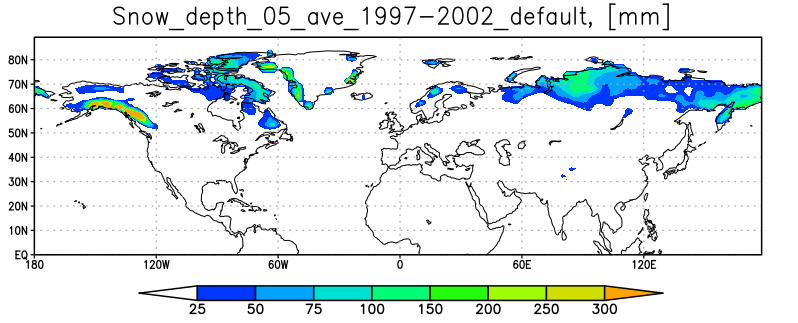
\includegraphics[width=1.1\linewidth]{Snow_depth_05_ave_1997-2002_default.png} \\ (а)}
    \end{minipage}
    \hfill
    \begin{minipage}[h]{0.49\linewidth}
        \center{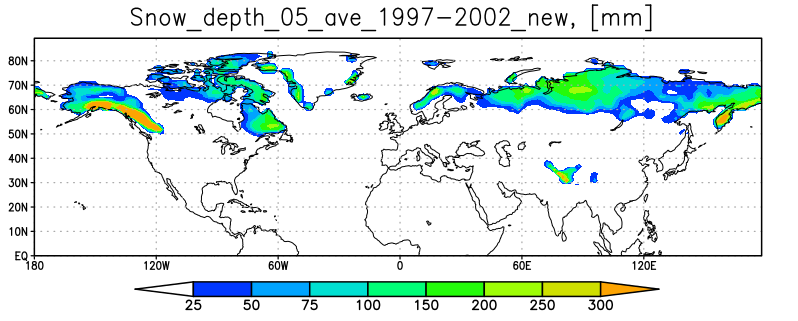
\includegraphics[width=1.1\linewidth]{Snow_depth_05_ave_1997-2002_new.png} \\ (б)}
    \end{minipage}
    \caption{Среднемесячная водно-эквивалентная толщина слоя снега по данным (а) исходной и (б) модифицированной версий модели ИВМ (месяц -- май) }
    \label{fig:image}
\end{figure}

Также нужно отметить, что более подробное описание почвенно- снежного блока привело к увеличению количества снега в целом (Рис. \ref{fig:imageSn}). Наибольшее различие между версиями наблюдается в весенние месяцы, при этом с июля по сентябрь различия минимальны. Это сравнение показывает, что реализованные процессы дают ощутимый вклад в образование снежного покрова.  В сравнении с данными наблюдений суммарная масса снега в случае модифицированной версии оказывается заметно завышенной, но, вместе с тем, описание площади, покрытой снегом, наоборот, улучшается. С точки зрения описания альбедо последний результат является положительным. Также можно отметить, что полученные результаты согласуется с тенденцией к завышению массы снега при более точном описании площади покрытия в ряде климатических моделей, участвующих в CMIP6, при использовании более подробного описания снега \cite{Mudryk2020}.

\begin{figure}[h]
    \begin{minipage}[h]{0.48\linewidth}
        \center{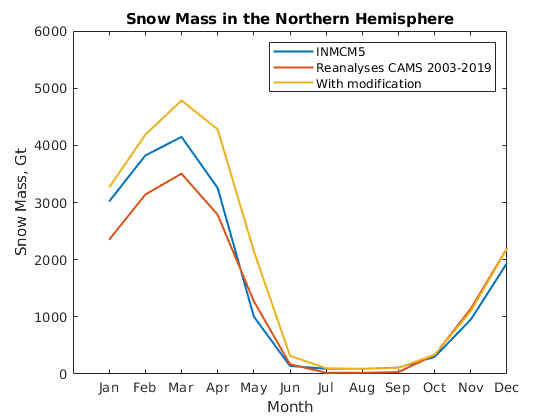
\includegraphics[width=1.1\linewidth]{snow_mass.png} \\ (а) }
    \end{minipage}
    \hfill
    \begin{minipage}[h]{0.51\linewidth}
        \center{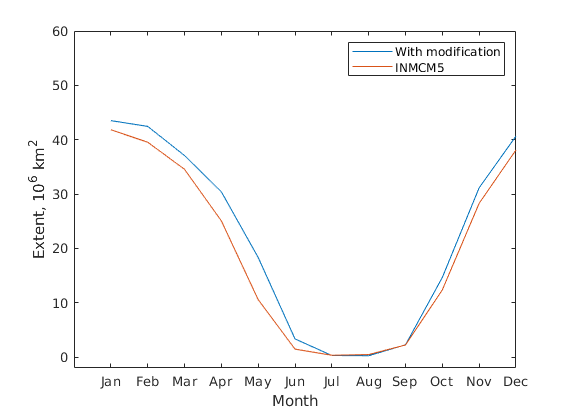
\includegraphics[width=1.1\linewidth]{snow_square.png} \\ (б) }
    \end{minipage}
    \caption{Годовой ход (а) массы снега и (б) площади, покрытой им, осредненные за 1997--2002 годы по данным исходной и модифицированной версий модели}
    \label{fig:imageSn}
\end{figure}

Другим важным результатом внесенных изменений в модель стала возможность проводить расчеты снежного альбедо с учетом метаморфизма снега, вызванного его старением, так как были добавлены недостающие модельные переменные.


\newpage
\section{Модель альбедо}

Полученные выше результаты позволяют перейти к вычислению альбедо. Для вычисления данной величины можно использовать как уже готовую модель, учитывающую описанные ранее факторы, так и некоторую параметризацию. 

\subsection{Описание радиационной модели SNICAR}
В качестве примера модели альбедо можно рассматривать локально-одномерную радиационную модель SNICAR (SNow-ICe-AErosole radiation model) \cite{Flanner2007}. Данная модель описывает вертикальный перенос излучения в слое снега с заданными профилями концентраций содержащихся в нем атмосферных аэрозолей, плотности среды и размеров снежных гранул, а одним из ее выходных данных является спектральное альбедо заснеженной поверхности. Данную модель можно использовать, например, для расчета альбедо заснеженной поверхности на этапе обработки данных из климатической модели. Внедрение данной модели в глобальную модель климата представляется достаточно сложной задачей. Однако, на ее основании можно построить параметризацию зависимости альбедо от основных параметров и уже ее внедрять в модель. Это может позволить проводить расчеты альбедо непосредственно в процессе работы глобальной модели и потенциально уточнить ее.

В любом случае, используя модель SNICAR или параметризацию, построенную на ее основе, а также зависимости, описывающие старение снега, концентрацию примесей в снегу и косинус солнечного зенитного угла и замыкаясь данными из модифицированной климатической модели ИВМ РАН, мы получаем полноценную модель альбедо.

\subsection{Построение параметризации альбедо на основе модели SNICAR}

Будем строить параметризацию альбедо от 3 переменных: эффективного радиуса снежного кристалла $r_e$, концентрации черного углерода в слое снега $C_{bc}$ и косинуса солнечного зенитного угла $coszen = cos(\theta)$ ($\theta$ -- солнечный зенитный угол). Предлагается строть параметризацию в два этапа: сначала получить зависимость от $r_e$ и $C_{bc}$, полагая $coszen = 1$, а затем уточнить ее за счет учета косинуса зенитного угла.

На первом этапе предлагается искать параметризацию альбедо в виде полинома от двух переменных:
\begin{equation}
    alb_1(r_e, C_{bc}) = \sum_{i,j = 0}^N \sigma_{i.j} r_e^i C_{bc}^j   \label{sys}  
\end{equation}
В ходе исследования \cite{mipt2020} было установлено, что наилучший результат получается в случае $N = 5$.

На втором этапе альбедо уточняется на основании эмпирической зависимости \cite{Saito2019}:
\begin{equation}
    alb(r_e, C_{bc}, coszen) = \alpha + (A + B \cdot \alpha^C) \left( \dfrac{1 - coszen}{1 + coszen} \right)^D     \label{sys}  
\end{equation}
Здесь $\alpha = alb_1(r_e, C_{bc})$ -- приближение с первого шага.

Параметры $\{ \sigma_{i.j} \}, A, B, C, D$ находятся на основании данных, полученных из результатов запусков модели SNICAR с различными значениями эффективного радиуса снежного кристалла, концентрации черного углерода и косинуса солнечного зенитного угла.

Полученная параметризация альбедо достаточно проста с вычислительной точки зрения, что делает возможным в будущем использование ее в глобальной климатической модели.

\subsection{Расчеты с использованием разработанной модели альбедо}

Результаты расчетов альбедо с помощью построенной модели показывают, что величина альбедо заснеженной поверхности, в целом, немного увеличилась (в среднем с $0.6$ до $0.80-0.85$) и приблизилась к результатам других моделей \cite{Flanner2007, Gueymard2019}. Важно отметить, что данная технология определена только для тех территорий, на которых лежит снег, в остальных местах необходимо пользоваться другими зависимостями.

\begin{figure}[h]
    \center{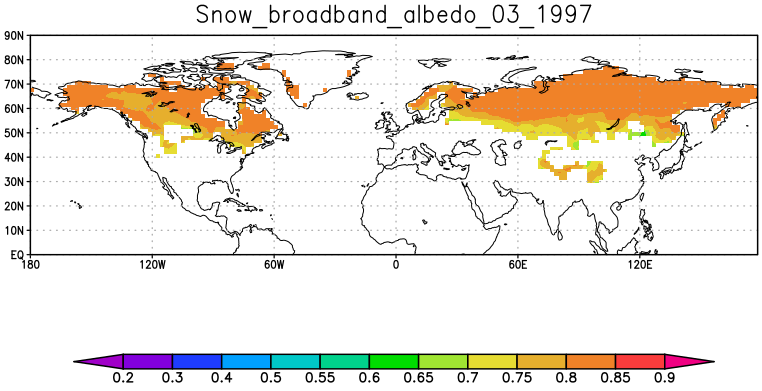
\includegraphics[scale=0.5]{Snow_albedo_03_1997.png}}
    \caption{Среднемесячное широкополосное альбедо заснеженной поверхности, рассчитанное с помощью построенной модели альбедо (март 1997 г.)}
    \label{fig:imageAlbOld}
\end{figure}

Полученные результаты расчета альбедо снега хорошо согласуются с данными Глобального реанализа CAMS (EAC4) Европейского центра среднесрочных прогнозов погоды.


\newpage
\section{Применение модели альбедо для вычисления радиационного форсинга}

Климат Земли и его чувствительность к различным воздействиям определяются естественными и антропогенными изменениями радиационного баланса Земли -- радиационным форсингом. Выпадая на снег, атмосферные аэрозоли уменьшают альбедо поверхности, что создает дополнительный радиационный форсинг. Это может приводить к более быстрому таянию снега и повышению приземной температуры в весенний сезон \cite{Chernenkov2021rus}. 

В данной главе оценивается радиационный форсинг, вызванный загрязнением снега черным углеродом. Дополнительный нагрев предлагается вычислять на основании изменения альбедо заснеженной поверхности и данных о приходящей радиации. Используя данные, полученные из модифицированной версии климатической модели ИВМ РАН, проведены расчеты с помощью построенной модели альбедо.

Определим необходимы переменные:
\begin{itemize}
    \item $\alpha_{0}$ и $\alpha_{soot}$ -- альбедо чистого и загрязненного снега соответственно,
    \item $\alpha^{vis}$ -- величина альбедо, соответствующая излучению в видимом диапазоне ($0.3-0.7$ мкм),
    \item $\alpha^{nir}$ -- величина альбедо, соответствующая излучению в ближнем ИК диапазоне ($0.7-5.0$ мкм),
    \item $\sigma$ -- доля области, покрытая снегом,
    \item $F_{sw}$ -- поток приходящей коротковолновой радиации.
\end{itemize}
Тогда форсинг можно оценить по следующей формуле:
\begin{equation}
    R = \sigma [ (\alpha_{0}^{vis} - \alpha_{soot}^{vis})F_{down}^{vis} + (\alpha_{0}^{nir} - \alpha_{soot}^{nir})F_{down}^{nir} ] \label{sysFORC}  
\end{equation}
При этом, потоки радиации $F_{down}^{vis}$ и $F_{down}^{nir}$ можно оценить следующим образом: 
\begin{equation}
    F_{down}^{vis} \approx F_{down}^{nir} \approx 0.5 \cdot F_{sw} \label{sys}  
\end{equation}

В формуле (\ref{sysFORC}) фигурируют альбедо и потоки радиации, только соответствующие видимому и ближнему инфракрасному диапазонам. Это оправдано, так как основной вклад в изменение спектрального альбедо из-за загрязнения снега приходится как раз на соответствующие диапазоны длин волн.

\begin{figure}[h]
    \center{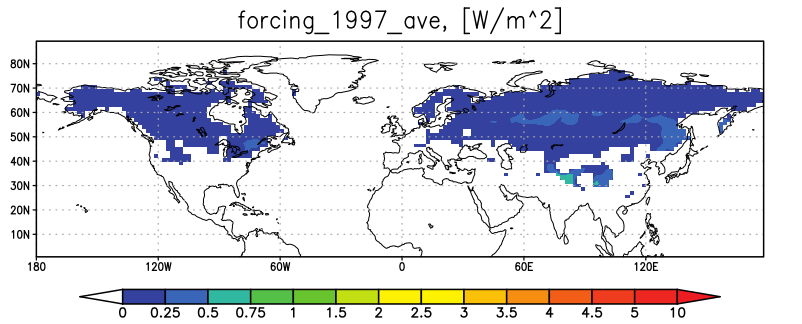
\includegraphics[scale=0.6]{forcing_1997.png}}
    \caption{Среднегодовой радиационный форсинг из-за загрязнения снега черным углеродом, рассчитанный с помощь построенной модели альбедо (1997 г.)}
    \label{fig:image}
\end{figure}

Нужно отметить, что учет структуры снега также оказывает влияние на радиационный форсинг. В случае старого снега форсинг от осадков черного углерода заметно выше, чем если бы весь снег считался свежевыпавшим. Такая добавка в среднем за год может составлять локально до $0.3$ Вт/м$^2$. 



%%%%%%%%%%%%%%%%%%%%%%%%%%%%%%%%%%%%%%%%%%%%%%%%%%%%%%%%%%%%%%%%%%%%%%%%%%%%%%%%%%%%%%%%%%%%%%%%%%%%%%%%%%%%%%%%%%%%%%%%%%%%%%%%%%%%%%%
\newpage
\section*{Заключение}
\addcontentsline{toc}{section}{\protect\numberline{}Заключение}

Данная магистерская диссертация является продолжением бакалаврской квалификационной работы \cite{Bak2019}. Основным результатом научно-исследовательской работы в магистратуре стала разработанная модель альбедо снега. 

В ходе работы были исследованы свойства альбедо заснеженной поверхности, получены зависимости, описывающие изменения величин, характеризующие эти свойства. Полученный результат можно использовать для внедрения блока расчета альбедо в модель климата. Другим приложением полученной модели является задача оценки радиационного форсинга от загрязнения снега атмосферными аэрозолями. Также в ходе работы был модифицирован почвенно-снежный блок глобальной климатической модели ИВМ РАН. 




%%%%%%%%%%%%%%%%%%%%%%%%%%%%%%%%%%%%%%%%%%%%%%%%%%%%%%%%%%%%%%%%%%%%%%%%%
\newpage
\phantomsection
\addcontentsline{toc}{section}{\protect\numberline{}Список литературы}
\bibliographystyle{gost2008}
\bibliography{biblio}







\end{document} 